\documentclass[1p]{elsarticle_modified}
%\bibliographystyle{elsarticle-num}

%\usepackage[colorlinks]{hyperref}
%\usepackage{abbrmath_seonhwa} %\Abb, \Ascr, \Acal ,\Abf, \Afrak
\usepackage{amsfonts}
\usepackage{amssymb}
\usepackage{amsmath}
\usepackage{amsthm}
\usepackage{scalefnt}
\usepackage{amsbsy}
\usepackage{kotex}
\usepackage{caption}
\usepackage{subfig}
\usepackage{color}
\usepackage{graphicx}
\usepackage{xcolor} %% white, black, red, green, blue, cyan, magenta, yellow
\usepackage{float}
\usepackage{setspace}
\usepackage{hyperref}

\usepackage{tikz}
\usetikzlibrary{arrows}

\usepackage{multirow}
\usepackage{array} % fixed length table
\usepackage{hhline}

%%%%%%%%%%%%%%%%%%%%%
\makeatletter
\renewcommand*\env@matrix[1][\arraystretch]{%
	\edef\arraystretch{#1}%
	\hskip -\arraycolsep
	\let\@ifnextchar\new@ifnextchar
	\array{*\c@MaxMatrixCols c}}
\makeatother %https://tex.stackexchange.com/questions/14071/how-can-i-increase-the-line-spacing-in-a-matrix
%%%%%%%%%%%%%%%

\usepackage[normalem]{ulem}

\newcommand{\msout}[1]{\ifmmode\text{\sout{\ensuremath{#1}}}\else\sout{#1}\fi}
%SOURCE: \msout is \stkout macro in https://tex.stackexchange.com/questions/20609/strikeout-in-math-mode

\newcommand{\cancel}[1]{
	\ifmmode
	{\color{red}\msout{#1}}
	\else
	{\color{red}\sout{#1}}
	\fi
}

\newcommand{\add}[1]{
	{\color{blue}\uwave{#1}}
}

\newcommand{\replace}[2]{
	\ifmmode
	{\color{red}\msout{#1}}{\color{blue}\uwave{#2}}
	\else
	{\color{red}\sout{#1}}{\color{blue}\uwave{#2}}
	\fi
}

\newcommand{\Sol}{\mathcal{S}} %segment
\newcommand{\D}{D} %diagram
\newcommand{\A}{\mathcal{A}} %arc


%%%%%%%%%%%%%%%%%%%%%%%%%%%%%5 test

\def\sl{\operatorname{\textup{SL}}(2,\Cbb)}
\def\psl{\operatorname{\textup{PSL}}(2,\Cbb)}
\def\quan{\mkern 1mu \triangleright \mkern 1mu}

\theoremstyle{definition}
\newtheorem{thm}{Theorem}[section]
\newtheorem{prop}[thm]{Proposition}
\newtheorem{lem}[thm]{Lemma}
\newtheorem{ques}[thm]{Question}
\newtheorem{cor}[thm]{Corollary}
\newtheorem{defn}[thm]{Definition}
\newtheorem{exam}[thm]{Example}
\newtheorem{rmk}[thm]{Remark}
\newtheorem{alg}[thm]{Algorithm}

\newcommand{\I}{\sqrt{-1}}
\begin{document}

%\begin{frontmatter}
%
%\title{Boundary parabolic representations of knots up to 8 crossings}
%
%%% Group authors per affiliation:
%\author{Yunhi Cho} 
%\address{Department of Mathematics, University of Seoul, Seoul, Korea}
%\ead{yhcho@uos.ac.kr}
%
%
%\author{Seonhwa Kim} %\fnref{s_kim}}
%\address{Center for Geometry and Physics, Institute for Basic Science, Pohang, 37673, Korea}
%\ead{ryeona17@ibs.re.kr}
%
%\author{Hyuk Kim}
%\address{Department of Mathematical Sciences, Seoul National University, Seoul 08826, Korea}
%\ead{hyukkim@snu.ac.kr}
%
%\author{Seokbeom Yoon}
%\address{Department of Mathematical Sciences, Seoul National University, Seoul, 08826,  Korea}
%\ead{sbyoon15@snu.ac.kr}
%
%\begin{abstract}
%We find all boundary parabolic representation of knots up to 8 crossings.
%
%\end{abstract}
%\begin{keyword}
%    \MSC[2010] 57M25 
%\end{keyword}
%
%\end{frontmatter}

%\linenumbers
%\tableofcontents
%
\newcommand\colored[1]{\textcolor{white}{\rule[-0.35ex]{0.8em}{1.4ex}}\kern-0.8em\color{red} #1}%
%\newcommand\colored[1]{\textcolor{white}{ #1}\kern-2.17ex	\textcolor{white}{ #1}\kern-1.81ex	\textcolor{white}{ #1}\kern-2.15ex\color{red}#1	}

{\Large $\underline{11a_{245}~(K11a_{245})}$}

\setlength{\tabcolsep}{10pt}
\renewcommand{\arraystretch}{1.6}
\vspace{1cm}\begin{tabular}{m{100pt}>{\centering\arraybackslash}m{274pt}}
\multirow{5}{120pt}{
	\centering
	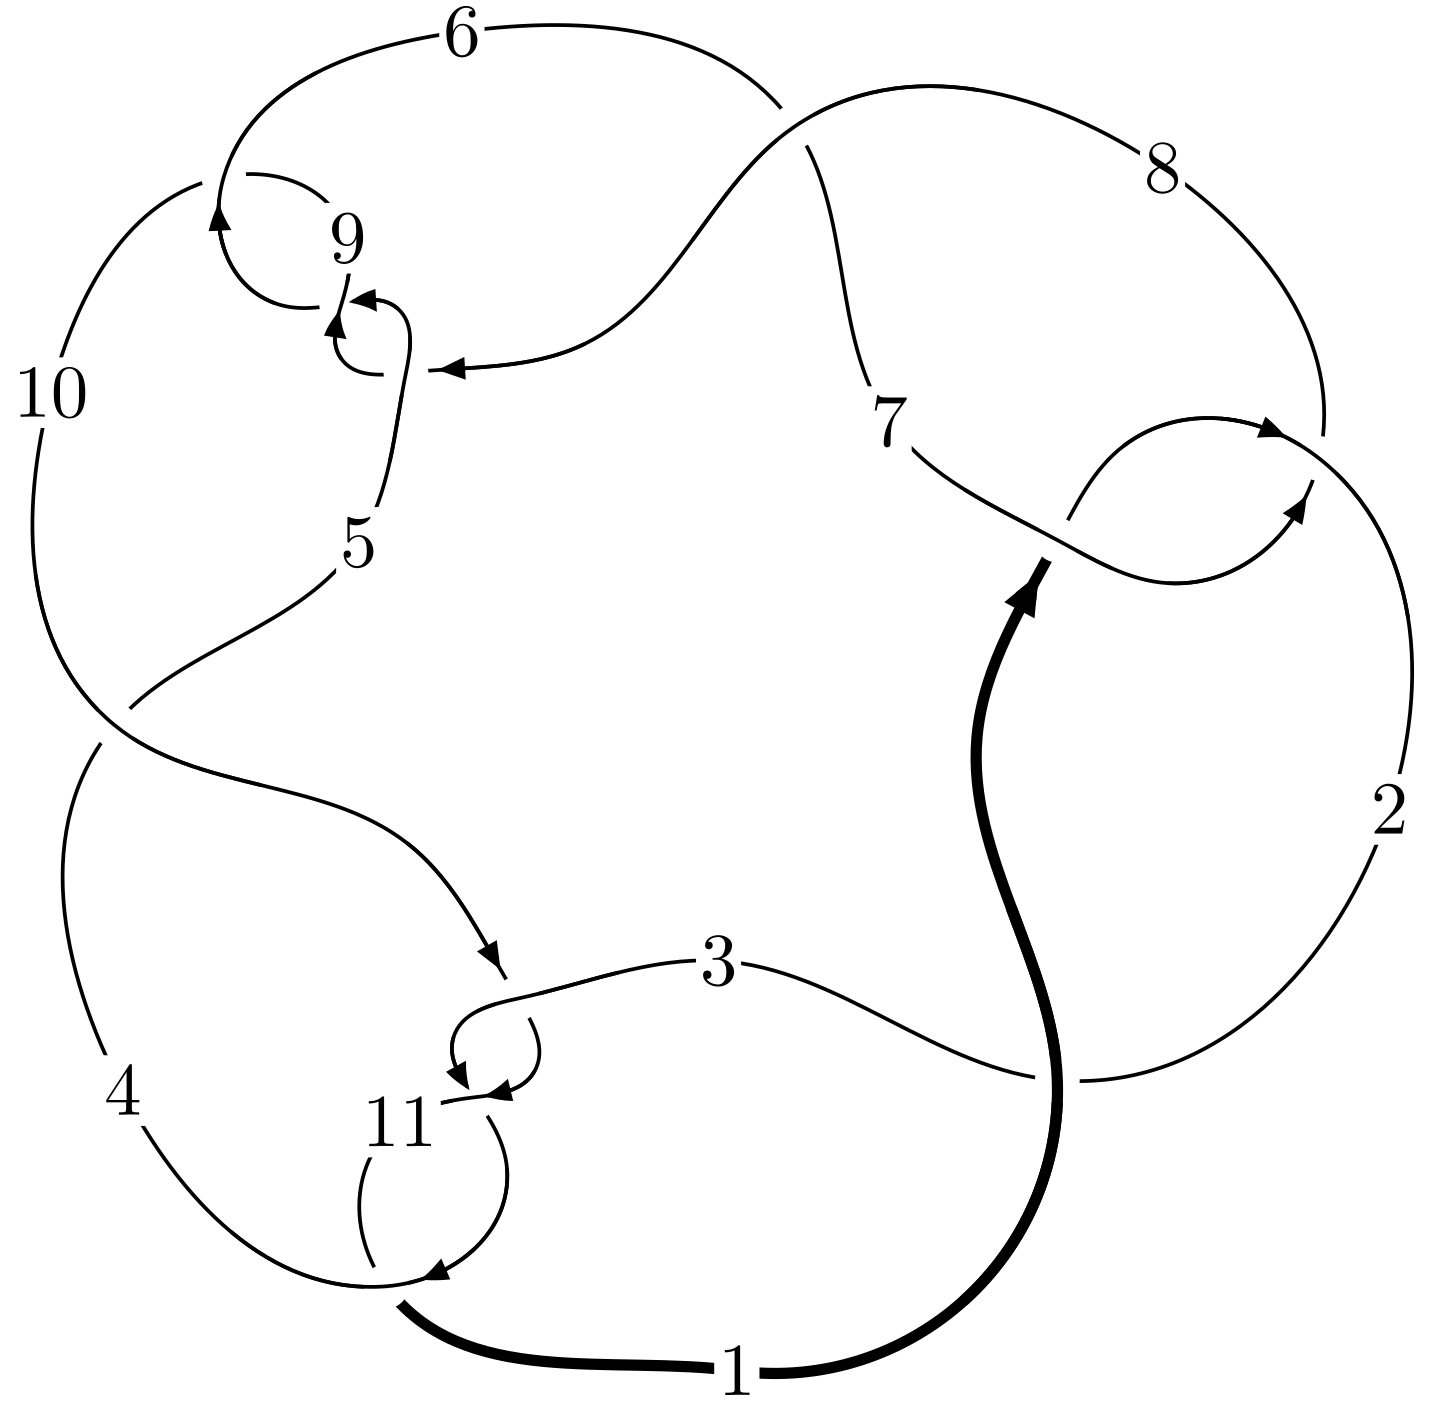
\includegraphics[width=112pt]{../../../GIT/diagram.site/Diagrams/png/494_11a_245.png}\\
\ \ \ A knot diagram\footnotemark}&
\allowdisplaybreaks
\textbf{Linearized knot diagam} \\
\cline{2-2}
 &
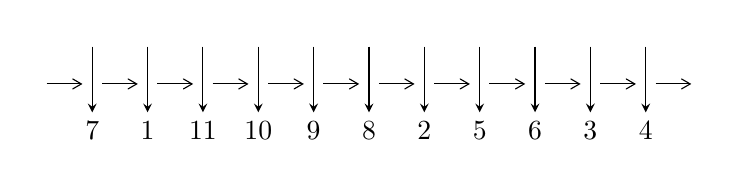
\begin{tikzpicture}[x=20pt, y=17pt]
	% nodes
	\node (C0) at (0, 0) {};
	\node (C1) at (1, 0) {};
	\node (C1U) at (1, +1) {};
	\node (C1D) at (1, -1) {7};

	\node (C2) at (2, 0) {};
	\node (C2U) at (2, +1) {};
	\node (C2D) at (2, -1) {1};

	\node (C3) at (3, 0) {};
	\node (C3U) at (3, +1) {};
	\node (C3D) at (3, -1) {11};

	\node (C4) at (4, 0) {};
	\node (C4U) at (4, +1) {};
	\node (C4D) at (4, -1) {10};

	\node (C5) at (5, 0) {};
	\node (C5U) at (5, +1) {};
	\node (C5D) at (5, -1) {9};

	\node (C6) at (6, 0) {};
	\node (C6U) at (6, +1) {};
	\node (C6D) at (6, -1) {8};

	\node (C7) at (7, 0) {};
	\node (C7U) at (7, +1) {};
	\node (C7D) at (7, -1) {2};

	\node (C8) at (8, 0) {};
	\node (C8U) at (8, +1) {};
	\node (C8D) at (8, -1) {5};

	\node (C9) at (9, 0) {};
	\node (C9U) at (9, +1) {};
	\node (C9D) at (9, -1) {6};

	\node (C10) at (10, 0) {};
	\node (C10U) at (10, +1) {};
	\node (C10D) at (10, -1) {3};

	\node (C11) at (11, 0) {};
	\node (C11U) at (11, +1) {};
	\node (C11D) at (11, -1) {4};
	\node (C12) at (12, 0) {};

	% arrows
	\draw[->,>={angle 60}]
	(C0) edge (C1) (C1) edge (C2) (C2) edge (C3) (C3) edge (C4) (C4) edge (C5) (C5) edge (C6) (C6) edge (C7) (C7) edge (C8) (C8) edge (C9) (C9) edge (C10) (C10) edge (C11) (C11) edge (C12) ;	\draw[->,>=stealth]
	(C1U) edge (C1D) (C2U) edge (C2D) (C3U) edge (C3D) (C4U) edge (C4D) (C5U) edge (C5D) (C6U) edge (C6D) (C7U) edge (C7D) (C8U) edge (C8D) (C9U) edge (C9D) (C10U) edge (C10D) (C11U) edge (C11D) ;
	\end{tikzpicture} \\
\hhline{~~} \\& 
\textbf{Solving Sequence} \\ \cline{2-2} 
 &
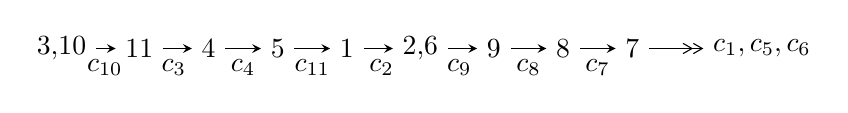
\begin{tikzpicture}[x=25pt, y=7pt]
	% node
	\node (A0) at (-1/8, 0) {3,10};
	\node (A1) at (1, 0) {11};
	\node (A2) at (2, 0) {4};
	\node (A3) at (3, 0) {5};
	\node (A4) at (4, 0) {1};
	\node (A5) at (81/16, 0) {2,6};
	\node (A6) at (49/8, 0) {9};
	\node (A7) at (57/8, 0) {8};
	\node (A8) at (65/8, 0) {7};
	\node (C1) at (1/2, -1) {$c_{10}$};
	\node (C2) at (3/2, -1) {$c_{3}$};
	\node (C3) at (5/2, -1) {$c_{4}$};
	\node (C4) at (7/2, -1) {$c_{11}$};
	\node (C5) at (9/2, -1) {$c_{2}$};
	\node (C6) at (45/8, -1) {$c_{9}$};
	\node (C7) at (53/8, -1) {$c_{8}$};
	\node (C8) at (61/8, -1) {$c_{7}$};
	\node (A9) at (10, 0) {$c_{1},c_{5},c_{6}$};

	% edge
	\draw[->,>=stealth]	
	(A0) edge (A1) (A1) edge (A2) (A2) edge (A3) (A3) edge (A4) (A4) edge (A5) (A5) edge (A6) (A6) edge (A7) (A7) edge (A8) ;
	\draw[->>,>={angle 60}]	
	(A8) edge (A9);
\end{tikzpicture} \\ 

\end{tabular} \\

\footnotetext{
The image of knot diagram is generated by the software ``\textbf{Draw programme}" developed by Andrew Bartholomew(\url{http://www.layer8.co.uk/maths/draw/index.htm\#Running-draw}), where we modified some parts for our purpose(\url{https://github.com/CATsTAILs/LinksPainter}).
}\phantom \\ \newline 
\centering \textbf{Ideals for irreducible components\footnotemark of $X_{\text{par}}$} 
 
\begin{align*}
I^u_{1}&=\langle 
b- u,\;- u^{12}+u^{11}+5 u^{10}-4 u^9-9 u^8+4 u^7+4 u^6+4 u^5+6 u^4-7 u^3-5 u^2+a- u-1,\\
\phantom{I^u_{1}}&\phantom{= \langle  }u^{14}- u^{13}-6 u^{12}+5 u^{11}+14 u^{10}-8 u^9-13 u^8-2 u^6+11 u^5+11 u^4-5 u^3-4 u^2-4 u-1\rangle \\
I^u_{2}&=\langle 
- u^{23}+8 u^{21}+\cdots+b+1,\;u^{22}-7 u^{20}+\cdots+a-1,\;u^{24}- u^{23}+\cdots+4 u^2+1\rangle \\
I^u_{3}&=\langle 
b+1,\;a,\;u-1\rangle \\
\\
\end{align*}
\raggedright * 3 irreducible components of $\dim_{\mathbb{C}}=0$, with total 39 representations.\\
\footnotetext{All coefficients of polynomials are rational numbers. But the coefficients are sometimes approximated in decimal forms when there is not enough margin.}
\newpage
\renewcommand{\arraystretch}{1}
\centering \section*{I. $I^u_{1}= \langle b- u,\;- u^{12}+u^{11}+\cdots+a-1,\;u^{14}- u^{13}+\cdots-4 u-1 \rangle$}
\flushleft \textbf{(i) Arc colorings}\\
\begin{tabular}{m{7pt} m{180pt} m{7pt} m{180pt} }
\flushright $a_{3}=$&$\begin{pmatrix}0\\u\end{pmatrix}$ \\
\flushright $a_{10}=$&$\begin{pmatrix}1\\0\end{pmatrix}$ \\
\flushright $a_{11}=$&$\begin{pmatrix}1\\u^2\end{pmatrix}$ \\
\flushright $a_{4}=$&$\begin{pmatrix}- u\\- u^3+u\end{pmatrix}$ \\
\flushright $a_{5}=$&$\begin{pmatrix}u^3-2 u\\- u^3+u\end{pmatrix}$ \\
\flushright $a_{1}=$&$\begin{pmatrix}- u^2+1\\- u^4+2 u^2\end{pmatrix}$ \\
\flushright $a_{2}=$&$\begin{pmatrix}u^5-2 u^3+u\\u^7-3 u^5+2 u^3+u\end{pmatrix}$ \\
\flushright $a_{6}=$&$\begin{pmatrix}u^{12}- u^{11}+\cdots+u+1\\u\end{pmatrix}$ \\
\flushright $a_{9}=$&$\begin{pmatrix}- u^{13}+u^{12}+\cdots- u+1\\- u^2\end{pmatrix}$ \\
\flushright $a_{8}=$&$\begin{pmatrix}- u^{13}+u^{12}+\cdots- u+1\\u^4-2 u^2\end{pmatrix}$ \\
\flushright $a_{7}=$&$\begin{pmatrix}u^{12}- u^{11}-5 u^{10}+4 u^9+9 u^8-5 u^7-4 u^6-6 u^4+3 u^3+5 u^2+1\\u^7-3 u^5+2 u^3+u\end{pmatrix}$\\ \flushright $a_{7}=$&$\begin{pmatrix}u^{12}- u^{11}-5 u^{10}+4 u^9+9 u^8-5 u^7-4 u^6-6 u^4+3 u^3+5 u^2+1\\u^7-3 u^5+2 u^3+u\end{pmatrix}$\\&\end{tabular}
\flushleft \textbf{(ii) Obstruction class $= -1$}\\~\\
\flushleft \textbf{(iii) Cusp Shapes $= -2 u^{12}-2 u^{11}+14 u^{10}+12 u^9-34 u^8-28 u^7+24 u^6+24 u^5+28 u^4+10 u^3-38 u^2-24 u-20$}\\~\\
\newpage\renewcommand{\arraystretch}{1}
\flushleft \textbf{(iv) u-Polynomials at the component}\newline \\
\begin{tabular}{m{50pt}|m{274pt}}
Crossings & \hspace{64pt}u-Polynomials at each crossing \\
\hline $$\begin{aligned}c_{1},c_{7}\end{aligned}$$&$\begin{aligned}
&u^{14}+3 u^{13}+\cdots+4 u+2
\end{aligned}$\\
\hline $$\begin{aligned}c_{2},c_{4},c_{6}\end{aligned}$$&$\begin{aligned}
&u^{14}+3 u^{13}+\cdots+20 u+4
\end{aligned}$\\
\hline $$\begin{aligned}c_{3},c_{5},c_{8}\\c_{9},c_{10},c_{11}\end{aligned}$$&$\begin{aligned}
&u^{14}- u^{13}+\cdots-4 u-1
\end{aligned}$\\
\hline
\end{tabular}\\~\\
\newpage\renewcommand{\arraystretch}{1}
\flushleft \textbf{(v) Riley Polynomials at the component}\newline \\
\begin{tabular}{m{50pt}|m{274pt}}
Crossings & \hspace{64pt}Riley Polynomials at each crossing \\
\hline $$\begin{aligned}c_{1},c_{7}\end{aligned}$$&$\begin{aligned}
&y^{14}-3 y^{13}+\cdots-20 y+4
\end{aligned}$\\
\hline $$\begin{aligned}c_{2},c_{4},c_{6}\end{aligned}$$&$\begin{aligned}
&y^{14}+13 y^{13}+\cdots-168 y+16
\end{aligned}$\\
\hline $$\begin{aligned}c_{3},c_{5},c_{8}\\c_{9},c_{10},c_{11}\end{aligned}$$&$\begin{aligned}
&y^{14}-13 y^{13}+\cdots-8 y+1
\end{aligned}$\\
\hline
\end{tabular}\\~\\
\newpage\flushleft \textbf{(vi) Complex Volumes and Cusp Shapes}
$$\begin{array}{c|c|c}  
\text{Solutions to }I^u_{1}& \I (\text{vol} + \sqrt{-1}CS) & \text{Cusp shape}\\
 \hline 
\begin{aligned}
u &= -0.029285 + 0.881113 I \\
a &= \phantom{-}0.03342 - 1.87376 I \\
b &= -0.029285 + 0.881113 I\end{aligned}
 & \phantom{-}8.40861 + 3.17852 I & -5.65702 - 2.68027 I \\ \hline\begin{aligned}
u &= -0.029285 - 0.881113 I \\
a &= \phantom{-}0.03342 + 1.87376 I \\
b &= -0.029285 - 0.881113 I\end{aligned}
 & \phantom{-}8.40861 - 3.17852 I & -5.65702 + 2.68027 I \\ \hline\begin{aligned}
u &= -1.276220 + 0.129179 I \\
a &= -2.13229 - 1.54329 I \\
b &= -1.276220 + 0.129179 I\end{aligned}
 & -5.86531 + 2.46178 I & -16.4162 - 2.9434 I \\ \hline\begin{aligned}
u &= -1.276220 - 0.129179 I \\
a &= -2.13229 + 1.54329 I \\
b &= -1.276220 - 0.129179 I\end{aligned}
 & -5.86531 - 2.46178 I & -16.4162 + 2.9434 I \\ \hline\begin{aligned}
u &= -1.284590 + 0.394747 I \\
a &= -0.34217 - 2.13508 I \\
b &= -1.284590 + 0.394747 I\end{aligned}
 & \phantom{-}0.58736 + 5.97274 I & -12.69846 - 3.76747 I \\ \hline\begin{aligned}
u &= -1.284590 - 0.394747 I \\
a &= -0.34217 + 2.13508 I \\
b &= -1.284590 - 0.394747 I\end{aligned}
 & \phantom{-}0.58736 - 5.97274 I & -12.69846 + 3.76747 I \\ \hline\begin{aligned}
u &= \phantom{-}1.364060 + 0.212940 I \\
a &= \phantom{-}1.10215 - 1.44780 I \\
b &= \phantom{-}1.364060 + 0.212940 I\end{aligned}
 & -8.69313 - 7.21786 I & -18.5779 + 6.6599 I \\ \hline\begin{aligned}
u &= \phantom{-}1.364060 - 0.212940 I \\
a &= \phantom{-}1.10215 + 1.44780 I \\
b &= \phantom{-}1.364060 - 0.212940 I\end{aligned}
 & -8.69313 + 7.21786 I & -18.5779 - 6.6599 I \\ \hline\begin{aligned}
u &= \phantom{-}1.38564\phantom{ +0.000000I} \\
a &= \phantom{-}1.62659\phantom{ +0.000000I} \\
b &= \phantom{-}1.38564\phantom{ +0.000000I}\end{aligned}
 & -11.4128\phantom{ +0.000000I} & -21.8330\phantom{ +0.000000I} \\ \hline\begin{aligned}
u &= \phantom{-}1.329060 + 0.410124 I \\
a &= \phantom{-}0.27755 - 1.96683 I \\
b &= \phantom{-}1.329060 + 0.410124 I\end{aligned}
 & -0.11168 - 12.47310 I & -13.5601 + 7.9056 I\\
 \hline 
 \end{array}$$\newpage$$\begin{array}{c|c|c}  
\text{Solutions to }I^u_{1}& \I (\text{vol} + \sqrt{-1}CS) & \text{Cusp shape}\\
 \hline 
\begin{aligned}
u &= \phantom{-}1.329060 - 0.410124 I \\
a &= \phantom{-}0.27755 + 1.96683 I \\
b &= \phantom{-}1.329060 - 0.410124 I\end{aligned}
 & -0.11168 + 12.47310 I & -13.5601 - 7.9056 I \\ \hline\begin{aligned}
u &= -0.150725 + 0.518889 I \\
a &= \phantom{-}0.285959 - 1.368390 I \\
b &= -0.150725 + 0.518889 I\end{aligned}
 & \phantom{-}1.00801 + 1.75508 I & -6.01712 - 6.20279 I \\ \hline\begin{aligned}
u &= -0.150725 - 0.518889 I \\
a &= \phantom{-}0.285959 + 1.368390 I \\
b &= -0.150725 - 0.518889 I\end{aligned}
 & \phantom{-}1.00801 - 1.75508 I & -6.01712 + 6.20279 I \\ \hline\begin{aligned}
u &= -0.290248\phantom{ +0.000000I} \\
a &= \phantom{-}0.924145\phantom{ +0.000000I} \\
b &= -0.290248\phantom{ +0.000000I}\end{aligned}
 & -0.639037\phantom{ +0.000000I} & -16.3130\phantom{ +0.000000I}\\
 \hline 
 \end{array}$$\newpage\newpage\renewcommand{\arraystretch}{1}
\centering \section*{II. $I^u_{2}= \langle - u^{23}+8 u^{21}+\cdots+b+1,\;u^{22}-7 u^{20}+\cdots+a-1,\;u^{24}- u^{23}+\cdots+4 u^2+1 \rangle$}
\flushleft \textbf{(i) Arc colorings}\\
\begin{tabular}{m{7pt} m{180pt} m{7pt} m{180pt} }
\flushright $a_{3}=$&$\begin{pmatrix}0\\u\end{pmatrix}$ \\
\flushright $a_{10}=$&$\begin{pmatrix}1\\0\end{pmatrix}$ \\
\flushright $a_{11}=$&$\begin{pmatrix}1\\u^2\end{pmatrix}$ \\
\flushright $a_{4}=$&$\begin{pmatrix}- u\\- u^3+u\end{pmatrix}$ \\
\flushright $a_{5}=$&$\begin{pmatrix}u^3-2 u\\- u^3+u\end{pmatrix}$ \\
\flushright $a_{1}=$&$\begin{pmatrix}- u^2+1\\- u^4+2 u^2\end{pmatrix}$ \\
\flushright $a_{2}=$&$\begin{pmatrix}u^5-2 u^3+u\\u^7-3 u^5+2 u^3+u\end{pmatrix}$ \\
\flushright $a_{6}=$&$\begin{pmatrix}- u^{22}+7 u^{20}+\cdots+5 u+1\\u^{23}-8 u^{21}+\cdots- u-1\end{pmatrix}$ \\
\flushright $a_{9}=$&$\begin{pmatrix}- u^{21}+8 u^{19}+\cdots+5 u+2\\u^{23}-7 u^{21}+\cdots- u-2\end{pmatrix}$ \\
\flushright $a_{8}=$&$\begin{pmatrix}u^{19}-6 u^{17}+\cdots+4 u+1\\2 u^{23}-15 u^{21}+\cdots- u-2\end{pmatrix}$ \\
\flushright $a_{7}=$&$\begin{pmatrix}- u^{16}+5 u^{14}+\cdots+4 u+1\\2 u^{23}-16 u^{21}+\cdots- u-2\end{pmatrix}$\\ \flushright $a_{7}=$&$\begin{pmatrix}- u^{16}+5 u^{14}+\cdots+4 u+1\\2 u^{23}-16 u^{21}+\cdots- u-2\end{pmatrix}$\\&\end{tabular}
\flushleft \textbf{(ii) Obstruction class $= -1$}\\~\\
\flushleft \textbf{(iii) Cusp Shapes $= -4 u^{20}+28 u^{18}+4 u^{17}-80 u^{16}-24 u^{15}+100 u^{14}+56 u^{13}-4 u^{12}-48 u^{11}-124 u^{10}-24 u^9+92 u^8+64 u^7+36 u^6-12 u^5-44 u^4-24 u^3-8 u^2-10$}\\~\\
\newpage\renewcommand{\arraystretch}{1}
\flushleft \textbf{(iv) u-Polynomials at the component}\newline \\
\begin{tabular}{m{50pt}|m{274pt}}
Crossings & \hspace{64pt}u-Polynomials at each crossing \\
\hline $$\begin{aligned}c_{1},c_{7}\end{aligned}$$&$\begin{aligned}
&(u^{12}- u^{11}- u^{10}+2 u^9+3 u^8-4 u^7-2 u^6+4 u^5+2 u^4-3 u^3- u^2+1)^2
\end{aligned}$\\
\hline $$\begin{aligned}c_{2},c_{4},c_{6}\end{aligned}$$&$\begin{aligned}
&(u^{12}+3 u^{11}+\cdots+2 u+1)^{2}
\end{aligned}$\\
\hline $$\begin{aligned}c_{3},c_{5},c_{8}\\c_{9},c_{10},c_{11}\end{aligned}$$&$\begin{aligned}
&u^{24}- u^{23}+\cdots+4 u^2+1
\end{aligned}$\\
\hline
\end{tabular}\\~\\
\newpage\renewcommand{\arraystretch}{1}
\flushleft \textbf{(v) Riley Polynomials at the component}\newline \\
\begin{tabular}{m{50pt}|m{274pt}}
Crossings & \hspace{64pt}Riley Polynomials at each crossing \\
\hline $$\begin{aligned}c_{1},c_{7}\end{aligned}$$&$\begin{aligned}
&(y^{12}-3 y^{11}+\cdots-2 y+1)^{2}
\end{aligned}$\\
\hline $$\begin{aligned}c_{2},c_{4},c_{6}\end{aligned}$$&$\begin{aligned}
&(y^{12}+13 y^{11}+\cdots+6 y+1)^{2}
\end{aligned}$\\
\hline $$\begin{aligned}c_{3},c_{5},c_{8}\\c_{9},c_{10},c_{11}\end{aligned}$$&$\begin{aligned}
&y^{24}-17 y^{23}+\cdots+8 y+1
\end{aligned}$\\
\hline
\end{tabular}\\~\\
\newpage\flushleft \textbf{(vi) Complex Volumes and Cusp Shapes}
$$\begin{array}{c|c|c}  
\text{Solutions to }I^u_{2}& \I (\text{vol} + \sqrt{-1}CS) & \text{Cusp shape}\\
 \hline 
\begin{aligned}
u &= -0.070751 + 0.894321 I \\
a &= -1.21139 + 1.52083 I \\
b &= \phantom{-}1.299300 - 0.409615 I\end{aligned}
 & \phantom{-}4.26829 + 7.80134 I & -9.63389 - 5.63981 I \\ \hline\begin{aligned}
u &= -0.070751 - 0.894321 I \\
a &= -1.21139 - 1.52083 I \\
b &= \phantom{-}1.299300 + 0.409615 I\end{aligned}
 & \phantom{-}4.26829 - 7.80134 I & -9.63389 + 5.63981 I \\ \hline\begin{aligned}
u &= -1.110590 + 0.134720 I \\
a &= \phantom{-}0.738153 + 0.451331 I \\
b &= \phantom{-}0.149210 - 0.343690 I\end{aligned}
 & -1.55013 + 0.71593 I & -8.04353 - 0.64874 I \\ \hline\begin{aligned}
u &= -1.110590 - 0.134720 I \\
a &= \phantom{-}0.738153 - 0.451331 I \\
b &= \phantom{-}0.149210 + 0.343690 I\end{aligned}
 & -1.55013 - 0.71593 I & -8.04353 + 0.64874 I \\ \hline\begin{aligned}
u &= -0.778878 + 0.387180 I \\
a &= -0.213014 + 0.440226 I \\
b &= \phantom{-}1.242510 + 0.071539 I\end{aligned}
 & -4.72717 - 0.35310 I & -18.6669 + 0.6298 I \\ \hline\begin{aligned}
u &= -0.778878 - 0.387180 I \\
a &= -0.213014 - 0.440226 I \\
b &= \phantom{-}1.242510 - 0.071539 I\end{aligned}
 & -4.72717 + 0.35310 I & -18.6669 - 0.6298 I \\ \hline\begin{aligned}
u &= \phantom{-}0.013292 + 0.856991 I \\
a &= \phantom{-}1.23384 + 1.58823 I \\
b &= -1.251930 - 0.421635 I\end{aligned}
 & \phantom{-}4.62532 - 1.48234 I & -8.84742 + 0.67542 I \\ \hline\begin{aligned}
u &= \phantom{-}0.013292 - 0.856991 I \\
a &= \phantom{-}1.23384 - 1.58823 I \\
b &= -1.251930 + 0.421635 I\end{aligned}
 & \phantom{-}4.62532 + 1.48234 I & -8.84742 - 0.67542 I \\ \hline\begin{aligned}
u &= \phantom{-}1.242510 + 0.071539 I \\
a &= -0.023283 - 0.340995 I \\
b &= -0.778878 + 0.387180 I\end{aligned}
 & -4.72717 - 0.35310 I & -18.6669 + 0.6298 I \\ \hline\begin{aligned}
u &= \phantom{-}1.242510 - 0.071539 I \\
a &= -0.023283 + 0.340995 I \\
b &= -0.778878 - 0.387180 I\end{aligned}
 & -4.72717 + 0.35310 I & -18.6669 - 0.6298 I\\
 \hline 
 \end{array}$$\newpage$$\begin{array}{c|c|c}  
\text{Solutions to }I^u_{2}& \I (\text{vol} + \sqrt{-1}CS) & \text{Cusp shape}\\
 \hline 
\begin{aligned}
u &= -0.321894 + 0.643464 I \\
a &= -0.65810 + 1.42592 I \\
b &= \phantom{-}1.279920 - 0.182904 I\end{aligned}
 & -3.36661 + 4.24921 I & -14.1765 - 6.9831 I \\ \hline\begin{aligned}
u &= -0.321894 - 0.643464 I \\
a &= -0.65810 - 1.42592 I \\
b &= \phantom{-}1.279920 + 0.182904 I\end{aligned}
 & -3.36661 - 4.24921 I & -14.1765 + 6.9831 I \\ \hline\begin{aligned}
u &= \phantom{-}1.279920 + 0.182904 I \\
a &= -0.443771 + 0.752880 I \\
b &= -0.321894 - 0.643464 I\end{aligned}
 & -3.36661 - 4.24921 I & -14.1765 + 6.9831 I \\ \hline\begin{aligned}
u &= \phantom{-}1.279920 - 0.182904 I \\
a &= -0.443771 - 0.752880 I \\
b &= -0.321894 + 0.643464 I\end{aligned}
 & -3.36661 + 4.24921 I & -14.1765 - 6.9831 I \\ \hline\begin{aligned}
u &= -1.213270 + 0.447486 I \\
a &= -0.537563 - 0.128960 I \\
b &= \phantom{-}1.263090 + 0.396551 I\end{aligned}
 & \phantom{-}0.75031 - 3.01307 I & -12.63175 + 2.63251 I \\ \hline\begin{aligned}
u &= -1.213270 - 0.447486 I \\
a &= -0.537563 + 0.128960 I \\
b &= \phantom{-}1.263090 - 0.396551 I\end{aligned}
 & \phantom{-}0.75031 + 3.01307 I & -12.63175 - 2.63251 I \\ \hline\begin{aligned}
u &= -1.251930 + 0.421635 I \\
a &= \phantom{-}0.704102 + 1.098600 I \\
b &= \phantom{-}0.013292 - 0.856991 I\end{aligned}
 & \phantom{-}4.62532 + 1.48234 I & -8.84742 - 0.67542 I \\ \hline\begin{aligned}
u &= -1.251930 - 0.421635 I \\
a &= \phantom{-}0.704102 - 1.098600 I \\
b &= \phantom{-}0.013292 + 0.856991 I\end{aligned}
 & \phantom{-}4.62532 - 1.48234 I & -8.84742 + 0.67542 I \\ \hline\begin{aligned}
u &= \phantom{-}1.263090 + 0.396551 I \\
a &= \phantom{-}0.492596 - 0.221226 I \\
b &= -1.213270 + 0.447486 I\end{aligned}
 & \phantom{-}0.75031 - 3.01307 I & -12.63175 + 2.63251 I \\ \hline\begin{aligned}
u &= \phantom{-}1.263090 - 0.396551 I \\
a &= \phantom{-}0.492596 + 0.221226 I \\
b &= -1.213270 - 0.447486 I\end{aligned}
 & \phantom{-}0.75031 + 3.01307 I & -12.63175 - 2.63251 I\\
 \hline 
 \end{array}$$\newpage$$\begin{array}{c|c|c}  
\text{Solutions to }I^u_{2}& \I (\text{vol} + \sqrt{-1}CS) & \text{Cusp shape}\\
 \hline 
\begin{aligned}
u &= \phantom{-}1.299300 + 0.409615 I \\
a &= -0.629315 + 1.115020 I \\
b &= -0.070751 - 0.894321 I\end{aligned}
 & \phantom{-}4.26829 - 7.80134 I & -9.63389 + 5.63981 I \\ \hline\begin{aligned}
u &= \phantom{-}1.299300 - 0.409615 I \\
a &= -0.629315 - 1.115020 I \\
b &= -0.070751 + 0.894321 I\end{aligned}
 & \phantom{-}4.26829 + 7.80134 I & -9.63389 - 5.63981 I \\ \hline\begin{aligned}
u &= \phantom{-}0.149210 + 0.343690 I \\
a &= \phantom{-}0.04774 + 2.58289 I \\
b &= -1.110590 - 0.134720 I\end{aligned}
 & -1.55013 - 0.71593 I & -8.04353 + 0.64874 I \\ \hline\begin{aligned}
u &= \phantom{-}0.149210 - 0.343690 I \\
a &= \phantom{-}0.04774 - 2.58289 I \\
b &= -1.110590 + 0.134720 I\end{aligned}
 & -1.55013 + 0.71593 I & -8.04353 - 0.64874 I\\
 \hline 
 \end{array}$$\newpage\newpage\renewcommand{\arraystretch}{1}
\centering \section*{III. $I^u_{3}= \langle b+1,\;a,\;u-1 \rangle$}
\flushleft \textbf{(i) Arc colorings}\\
\begin{tabular}{m{7pt} m{180pt} m{7pt} m{180pt} }
\flushright $a_{3}=$&$\begin{pmatrix}0\\1\end{pmatrix}$ \\
\flushright $a_{10}=$&$\begin{pmatrix}1\\0\end{pmatrix}$ \\
\flushright $a_{11}=$&$\begin{pmatrix}1\\1\end{pmatrix}$ \\
\flushright $a_{4}=$&$\begin{pmatrix}-1\\0\end{pmatrix}$ \\
\flushright $a_{5}=$&$\begin{pmatrix}-1\\0\end{pmatrix}$ \\
\flushright $a_{1}=$&$\begin{pmatrix}0\\1\end{pmatrix}$ \\
\flushright $a_{2}=$&$\begin{pmatrix}0\\1\end{pmatrix}$ \\
\flushright $a_{6}=$&$\begin{pmatrix}0\\-1\end{pmatrix}$ \\
\flushright $a_{9}=$&$\begin{pmatrix}1\\-1\end{pmatrix}$ \\
\flushright $a_{8}=$&$\begin{pmatrix}0\\-1\end{pmatrix}$ \\
\flushright $a_{7}=$&$\begin{pmatrix}0\\-1\end{pmatrix}$\\ \flushright $a_{7}=$&$\begin{pmatrix}0\\-1\end{pmatrix}$\\&\end{tabular}
\flushleft \textbf{(ii) Obstruction class $= 1$}\\~\\
\flushleft \textbf{(iii) Cusp Shapes $= -12$}\\~\\
\newpage\renewcommand{\arraystretch}{1}
\flushleft \textbf{(iv) u-Polynomials at the component}\newline \\
\begin{tabular}{m{50pt}|m{274pt}}
Crossings & \hspace{64pt}u-Polynomials at each crossing \\
\hline $$\begin{aligned}c_{1},c_{2},c_{4}\\c_{6},c_{7}\end{aligned}$$&$\begin{aligned}
&u
\end{aligned}$\\
\hline $$\begin{aligned}c_{3},c_{8},c_{9}\end{aligned}$$&$\begin{aligned}
&u+1
\end{aligned}$\\
\hline $$\begin{aligned}c_{5},c_{10},c_{11}\end{aligned}$$&$\begin{aligned}
&u-1
\end{aligned}$\\
\hline
\end{tabular}\\~\\
\newpage\renewcommand{\arraystretch}{1}
\flushleft \textbf{(v) Riley Polynomials at the component}\newline \\
\begin{tabular}{m{50pt}|m{274pt}}
Crossings & \hspace{64pt}Riley Polynomials at each crossing \\
\hline $$\begin{aligned}c_{1},c_{2},c_{4}\\c_{6},c_{7}\end{aligned}$$&$\begin{aligned}
&y
\end{aligned}$\\
\hline $$\begin{aligned}c_{3},c_{5},c_{8}\\c_{9},c_{10},c_{11}\end{aligned}$$&$\begin{aligned}
&y-1
\end{aligned}$\\
\hline
\end{tabular}\\~\\
\newpage\flushleft \textbf{(vi) Complex Volumes and Cusp Shapes}
$$\begin{array}{c|c|c}  
\text{Solutions to }I^u_{3}& \I (\text{vol} + \sqrt{-1}CS) & \text{Cusp shape}\\
 \hline 
\begin{aligned}
u &= \phantom{-}1.00000\phantom{ +0.000000I} \\
a &= \phantom{-0.000000 } 0 \\
b &= -1.00000\phantom{ +0.000000I}\end{aligned}
 & -3.28987\phantom{ +0.000000I} & -12.0000\phantom{ +0.000000I}\\
 \hline 
 \end{array}$$\newpage
\newpage\renewcommand{\arraystretch}{1}
\centering \section*{ IV. u-Polynomials}
\begin{tabular}{m{50pt}|m{274pt}}
Crossings & \hspace{64pt}u-Polynomials at each crossing \\
\hline $$\begin{aligned}c_{1},c_{7}\end{aligned}$$&$\begin{aligned}
&u(u^{12}- u^{11}- u^{10}+2 u^9+3 u^8-4 u^7-2 u^6+4 u^5+2 u^4-3 u^3- u^2+1)^2\\
&\cdot(u^{14}+3 u^{13}+\cdots+4 u+2)
\end{aligned}$\\
\hline $$\begin{aligned}c_{2},c_{4},c_{6}\end{aligned}$$&$\begin{aligned}
&u(u^{12}+3 u^{11}+\cdots+2 u+1)^{2}(u^{14}+3 u^{13}+\cdots+20 u+4)
\end{aligned}$\\
\hline $$\begin{aligned}c_{3},c_{8},c_{9}\end{aligned}$$&$\begin{aligned}
&(u+1)(u^{14}- u^{13}+\cdots-4 u-1)(u^{24}- u^{23}+\cdots+4 u^2+1)
\end{aligned}$\\
\hline $$\begin{aligned}c_{5},c_{10},c_{11}\end{aligned}$$&$\begin{aligned}
&(u-1)(u^{14}- u^{13}+\cdots-4 u-1)(u^{24}- u^{23}+\cdots+4 u^2+1)
\end{aligned}$\\
\hline
\end{tabular}\newpage\renewcommand{\arraystretch}{1}
\centering \section*{ V. Riley Polynomials}
\begin{tabular}{m{50pt}|m{274pt}}
Crossings & \hspace{64pt}Riley Polynomials at each crossing \\
\hline $$\begin{aligned}c_{1},c_{7}\end{aligned}$$&$\begin{aligned}
&y(y^{12}-3 y^{11}+\cdots-2 y+1)^{2}(y^{14}-3 y^{13}+\cdots-20 y+4)
\end{aligned}$\\
\hline $$\begin{aligned}c_{2},c_{4},c_{6}\end{aligned}$$&$\begin{aligned}
&y(y^{12}+13 y^{11}+\cdots+6 y+1)^{2}(y^{14}+13 y^{13}+\cdots-168 y+16)
\end{aligned}$\\
\hline $$\begin{aligned}c_{3},c_{5},c_{8}\\c_{9},c_{10},c_{11}\end{aligned}$$&$\begin{aligned}
&(y-1)(y^{14}-13 y^{13}+\cdots-8 y+1)(y^{24}-17 y^{23}+\cdots+8 y+1)
\end{aligned}$\\
\hline
\end{tabular}
\vskip 2pc
\end{document}